	\section{Resultados experimentales}
	\label{sec:resultados}

	\newcommand{\prefacnota}{\footnote{
		Índice que representa la granularidad del entorno descrita en el \refcruzada{Apartado}{sec:espacio}
	}}

\subsection{Ajuste paramétrico}
Los parámetros empleados por el algoritmo en todas las ejecuciones mostradas en éste documento se encuentran recogidos en la \refcruzada{Tabla}{tabla:1}
\begin{savenotes}
	\begin{table}[]
	   	\centering
	    \caption{Parámetros del algoritmo y sus respectivos valores}
		\begin{tabular}{|l|c|}
			\hline
			Parameter                      & Exploit Mode / Explore Mode                      \\
			\hline
			Num. Robots                    & 50                                               \\
			$\omega$ (inertia)             & 0.5 / 1                                          \\
			$c_1$ (self learning factor)   & 0.5                                              \\
			$c_2$ (social learning factor) & 0.5 / 1                                          \\
			$c_d$ (evaporation factor)     & 0.5                                              \\
			$c_a$ (superposition factor)   & 0.5                                              \\
			Iteraciones Maximas            & 600                                              \\
			Exploring iterations           & 20                                               \\
			Max velocity                   & 1                                                \\
			Precision Factor\prefacnota    & 20                                               \\ \hline
		\end{tabular}
    	\label{tabla:1}
	\end{table}
\end{savenotes}


	
	\subsection{Variaciones en la función objetivo}
	En el artículo original~\cite{initialPaper} únicamente se utilizaba una función lineal, cuyo punto máximo se hallaba en el $(8,8)$ de una cuadrícula de $10\times10$, esto es así debido a que el enfoque de sus autores no era la optimización de la misma, sino una futura implementación a nivel físico, donde la función objetivo sería implementada mediante una señal (acústica o lumínica). Para analizar el potencial de éste sistema, se han probado algunas funciones de optimización conocidas, recopiladas en~\cite{WebFuncionesOptimizacion}.
	
	\subsubsection{Función de Ackley} Propuesta en~\cite{AckleyFunction} se define como
	\[ f(x,y)=-20 \cdot \exp[-0.2 \cdot \sqrt{0.5 \cdot (x^2 + y^2)}] - \exp[0.5 ( \cos(2 \pi x)
	+ \cos(2 \pi y))] + e + 20\]
	Al estar pensada para minimización y definida en el intervalo $[-5,5]$, consideramos la función $f'(x,y)=(-1)\cdot f(x-5, y-5)$. Se trata de una función no convexa, con una gran cantidad de máximos locales, como puede apreciarse en la \refcruzada{Fig.}{fig:2}, siendo el máximo absoluto el punto $(5,5)$.
	
	\begin{figure}[htbp]
	    \centering
	    \subfigure[Gráfica sobre 3 ejes]{
	    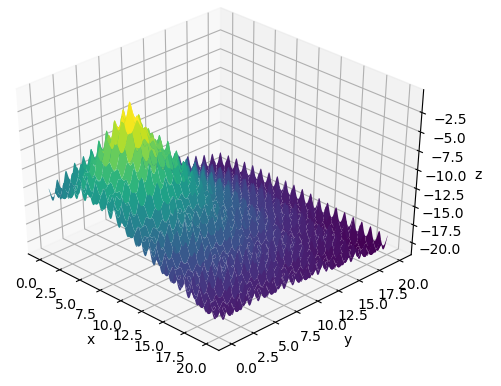
\includegraphics[width=0.4\textwidth]{funciones/graficas_ackley}
	    }
	    \subfigure[Curvas de nivel]{
	    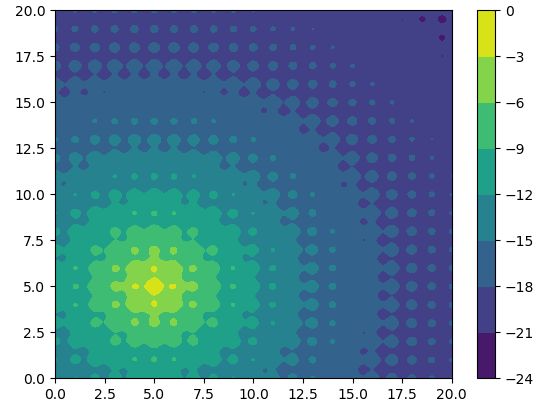
\includegraphics[width=0.5\textwidth]{funciones/graficas_ackley_contorno}
	    }
	    \caption{Representación de la función Ackley modificada para $x,y\in[0,20]$}
	    \label{fig:2}
	\end{figure}
	
	Los resultados tras 1\,300 iteraciones es el de la \refcruzada{Fig.}{fig:3}, como puede verse, se produce una convergencia casi total hace el punto $(5,5)$, sin embargo el mapa de feromonas construido no es útil, pues prácticamente todos los valores son de módulo cero.
	
	\begin{figure}[htbp]
	    \centering
	    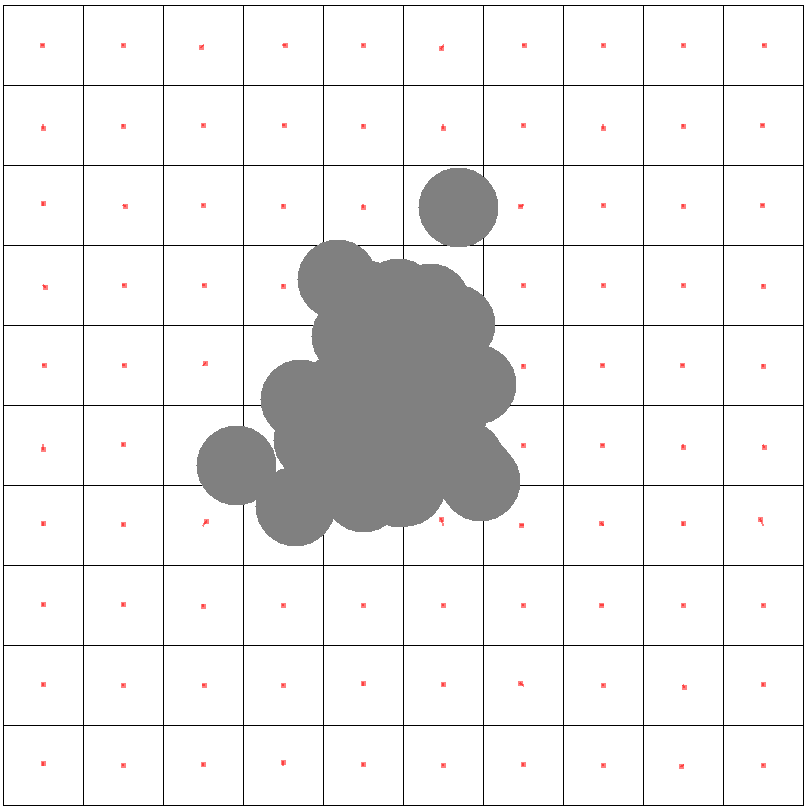
\includegraphics[width=0.4\textwidth]{funciones/Resultado_ackley}
	    \caption{Resultados experimentales empleando la función Ackley}
	    \label{fig:3}
	\end{figure}
	
	\subsubsection{Función de Himmelblau} Propuesta en~\cite{HimmelblauFunction} se define para el caso de una maximización como
	\[  f(x,y)=-(x^2 + y - 11)^2 - (x + y^2 - 7)^2  \]
	Contiene una meseta en la parte superior, por lo que no existe una única solución (ver \refcruzada{Fig.}{fig:4}).
	En cuanto a los resultados obtenidos, mostrados en la \refcruzada{Fig.}{fig:5}, el sistema no es capaz de converger, en su lugar, se forman 3 grupos de agentes en torno a los 4 posibles óptimos que tiene la función (ver~\cite{WebFuncionesOptimizacion} para más información sobre ésta función)
	
	
	\begin{figure}[htbp]
	    \centering
	    \subfigure[Gráfica sobre 3 ejes]{
	    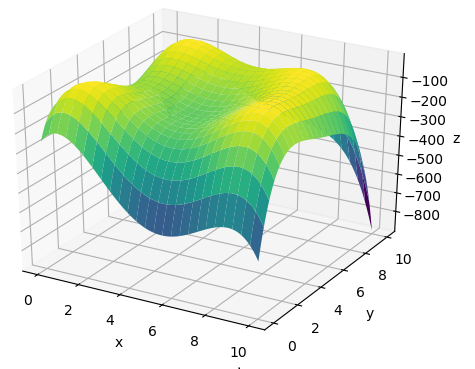
\includegraphics[width=0.4\textwidth]{funciones/graficas_himmelblau}
	    }
	    \subfigure[Curvas de nivel]{
	    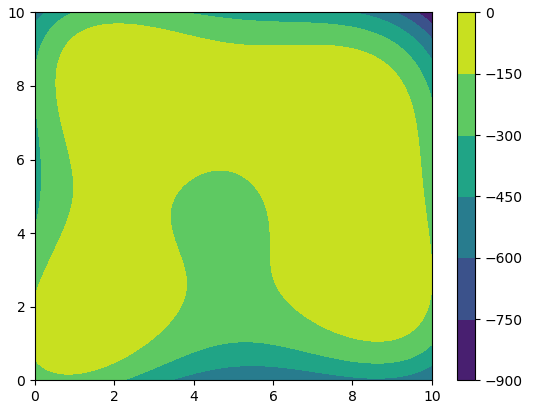
\includegraphics[width=0.5\textwidth]{funciones/graficas_himmelblau_contorno}
	    }
	    \caption{Representación de la función Himmelblau modificada para $x,y\in[0,10]$}
	    \label{fig:4}
	\end{figure}
	
	\begin{figure}[htbp]
	    \centering
	    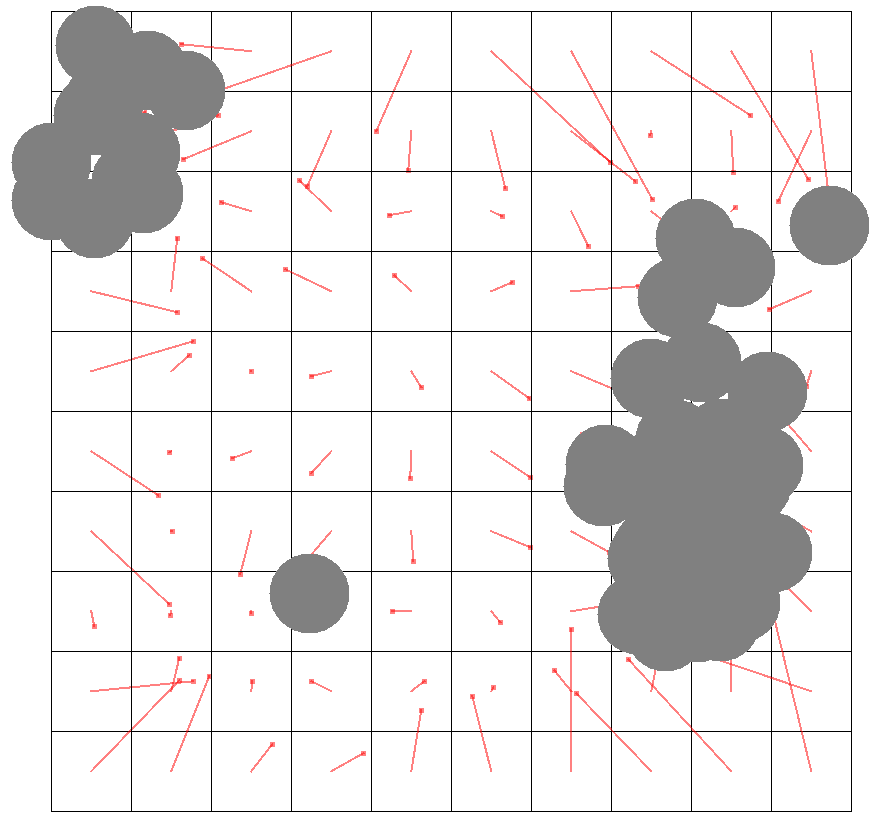
\includegraphics[width=0.4\textwidth]{funciones/Resultados_himmelblau_10x10}
	    \caption{Resultados experimentales empleando la función Himmelblau sobre una cuadricula $10\times10$}
	    \label{fig:5}
	\end{figure}
	
	\comment{
	\subsubsection{Función Lineal}
	$f(x,y)=-(x-g_x)^2 - (y - g_y)^2 + 700$; con máximo en $(g_x,g_y)$
	}
	\subsection{Pruebas con obstáculos}
	
	En esta sección, se ha tomado la función objetivo lineal de~\cite{initialPaper} añadiendo celdas de color negro que representan posiciones del espacio que las partículas no pueden atravesar.
	
	En estas ejecuciones, se suceden 20 iteraciones de exploración cada vez que el agente no sea capaz de encontrar una solución local que mejore sus resultados. Observamos convergencia tras 600 iteraciones.
	
	En el primer obstáculo, al ser de un tamaño no demasiado grande (\refcruzada{Fig.}{fig:6}), todos los agentes logran evitarlo y converger hacia la meta exitosamente.
	
	%%%%%%%%%%%%%%%
	% Obstáculo 1 %
	%%%%%%%%%%%%%%%
	\begin{figure}[htbp]
	    \centering
	    %        \subfigure[iteraciones=0]{
	    %        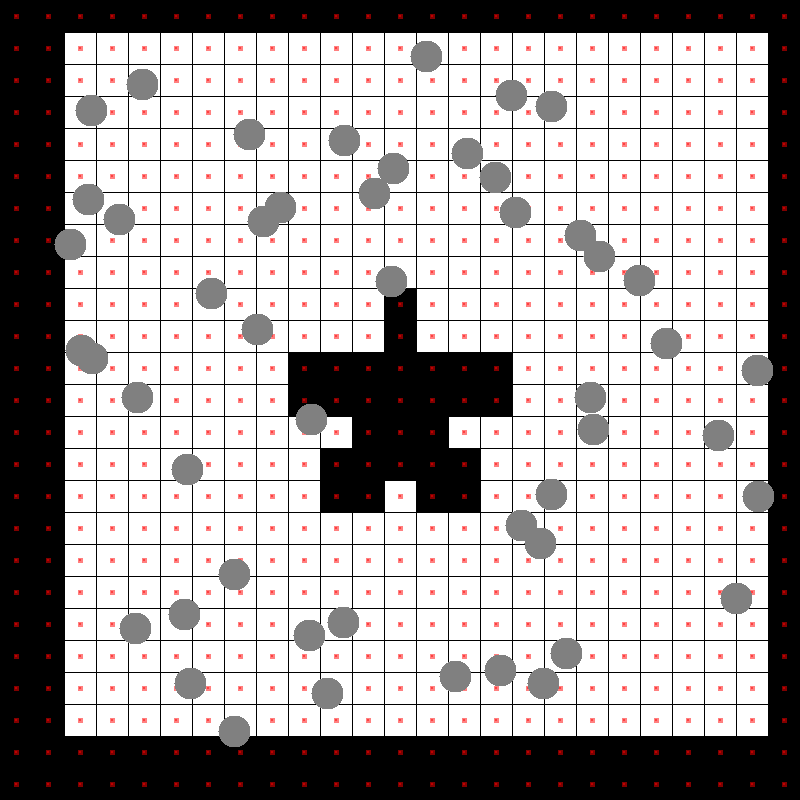
\includegraphics[width=0.3\textwidth]{obstaculos/obstaculo1_inicio}
	    %        }
	    \subfigure[iteraciones=20]{
	    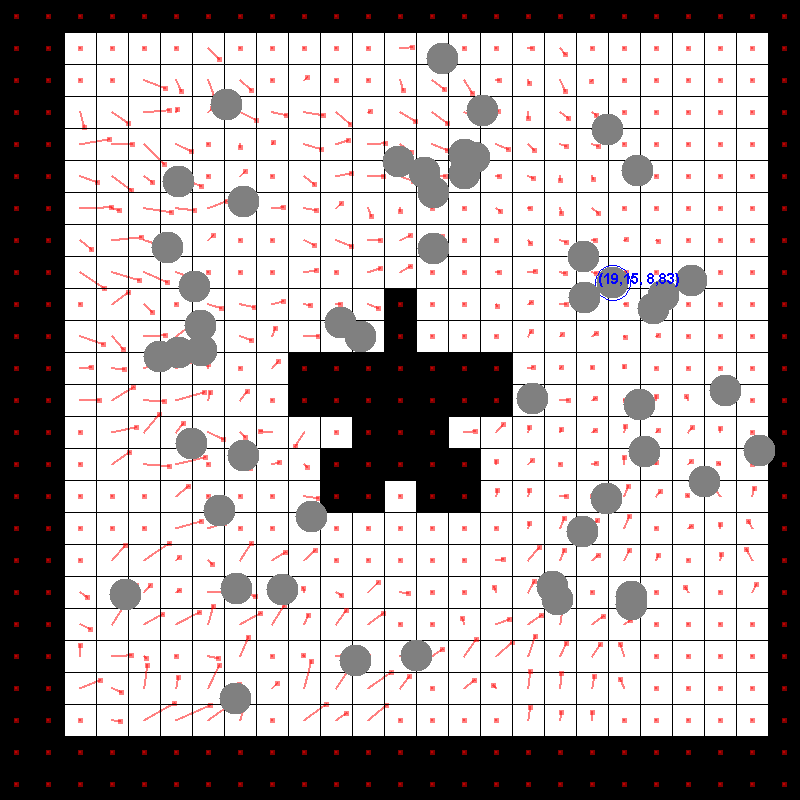
\includegraphics[width=0.3\textwidth]{obstaculos/obstaculo1_tras23iteraciones_exploremode}
	    }
	    \subfigure[iteraciones=40]{
	    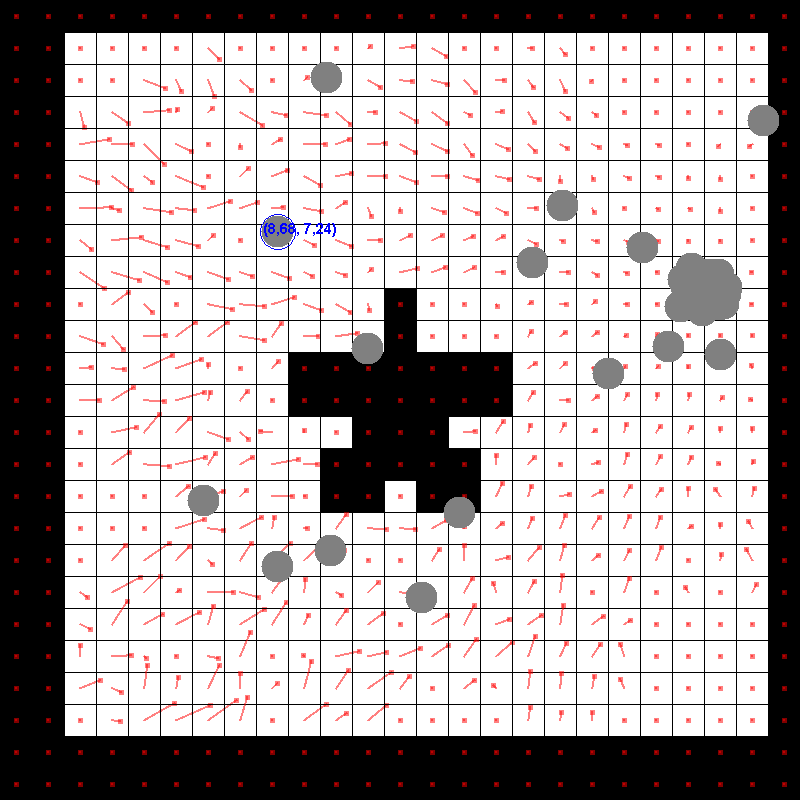
\includegraphics[width=0.3\textwidth]{obstaculos/obstaculo1_tras40iteraciones.png}
	    }
	    \subfigure[Iteraciones=600]{
	    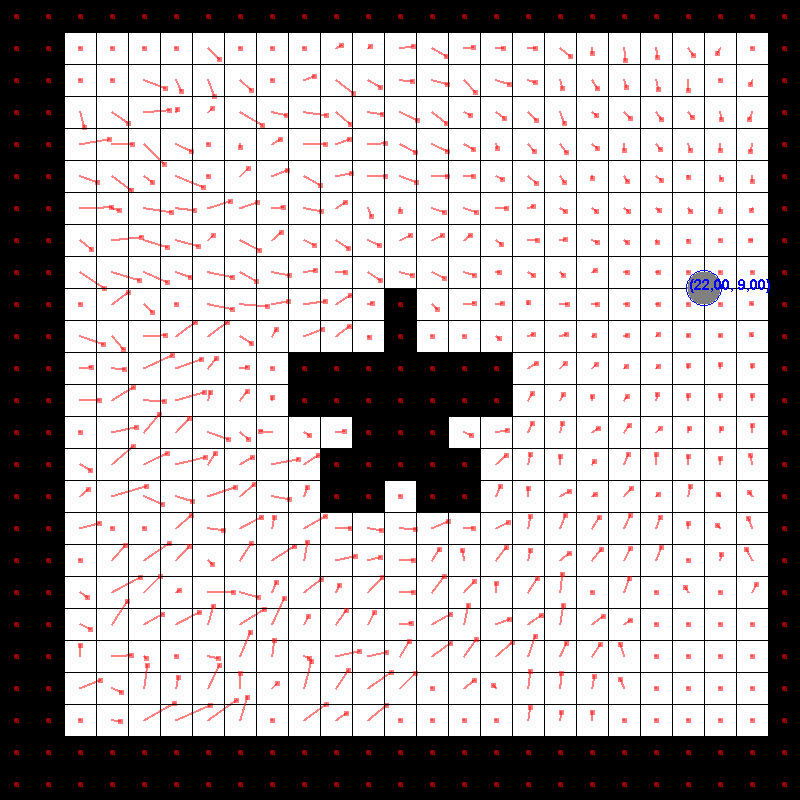
\includegraphics[width=0.3\textwidth]{obstaculos/obstaculo1_inicio_tras_600_iteraciones}
	    }
	    \caption{Ejecución con un obstáculo convexo}
	    \label{fig:6}
	\end{figure}
	
	Si empleamos un obstáculo mayor, como el de la \refcruzada{Fig.}{fig:8} los agentes no son capaces de sortear por completo el obstáculo inferior, pues los movimientos necesarios para recorrerlo y evitarlo son mucho mayores. Se necesita de una técnica con mayor inteligencia.
	
	%%%%%%%%%%%%%%%
	% Obstáculo 3 %
	%%%%%%%%%%%%%%%
	\begin{figure}[htbp]
	    \centering
	    %	\subfigure[iteraciones=0]{
	    %		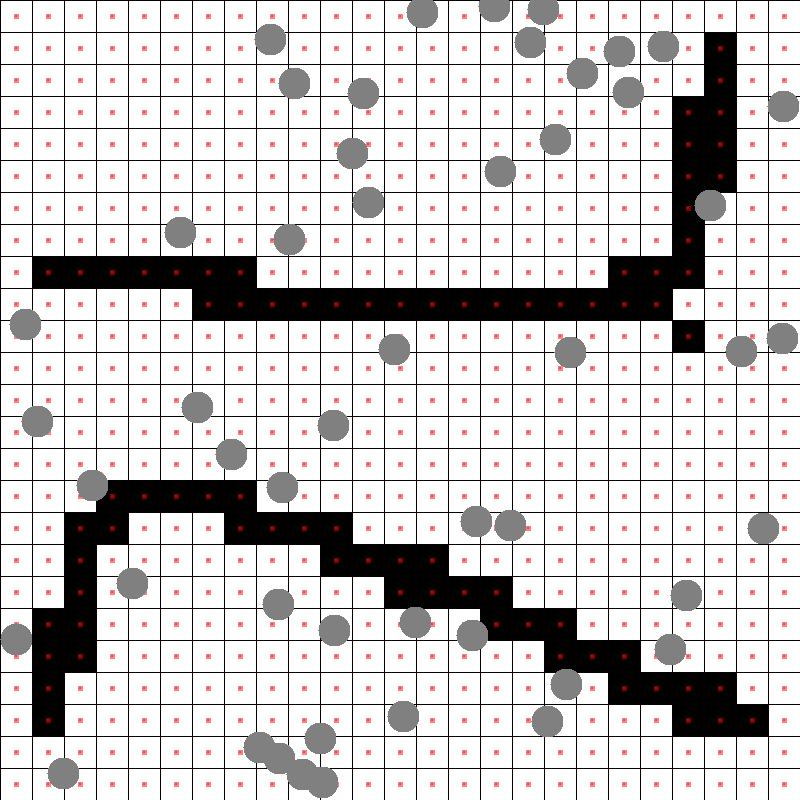
\includegraphics[width=0.4\textwidth]{obstaculos/obstaculo2_inicio}
	    %	}
	    \subfigure[iteraciones=20]{
	    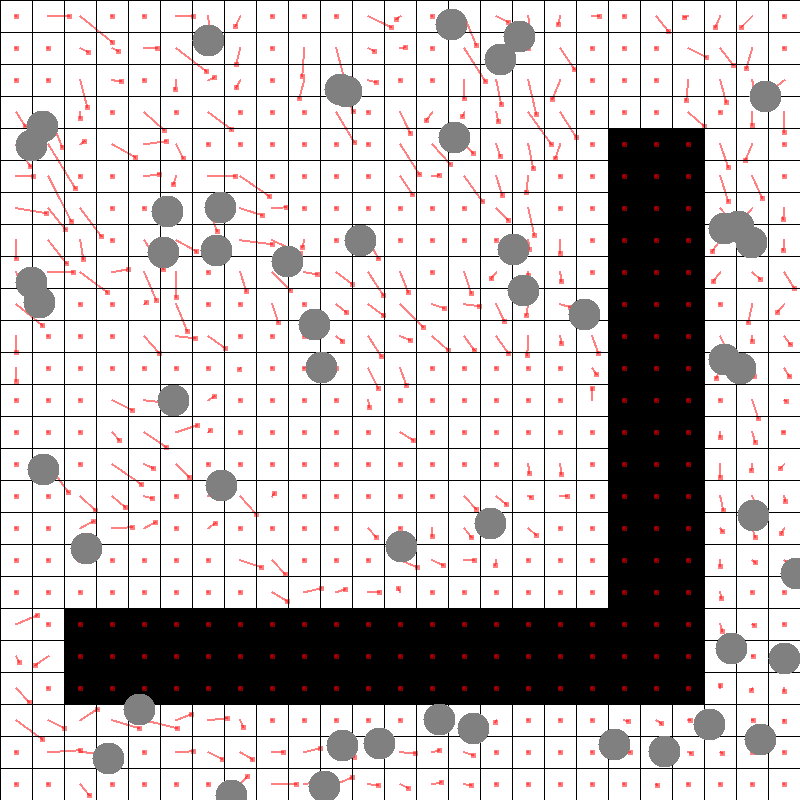
\includegraphics[width=0.3\textwidth]{obstaculos/obstaculo3_tras20iteraciones_exploremode}
	    }
	    \subfigure[iteraciones=40]{
	    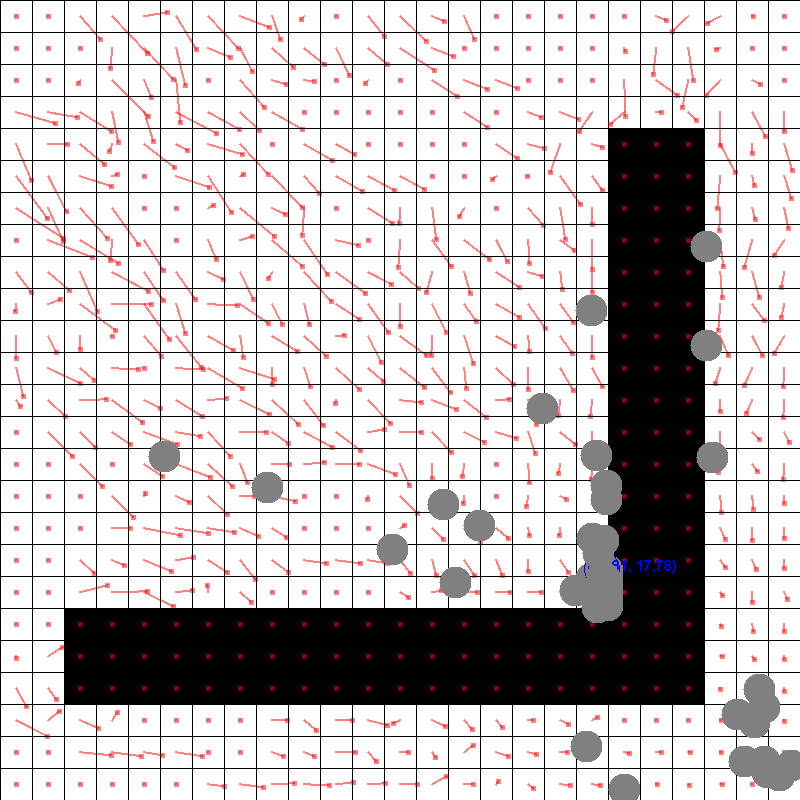
\includegraphics[width=0.3\textwidth]{obstaculos/obstaculo3_tras49iteraciones_exploitmode}
	    }
	    \subfigure[Iteraciones=600]{
	    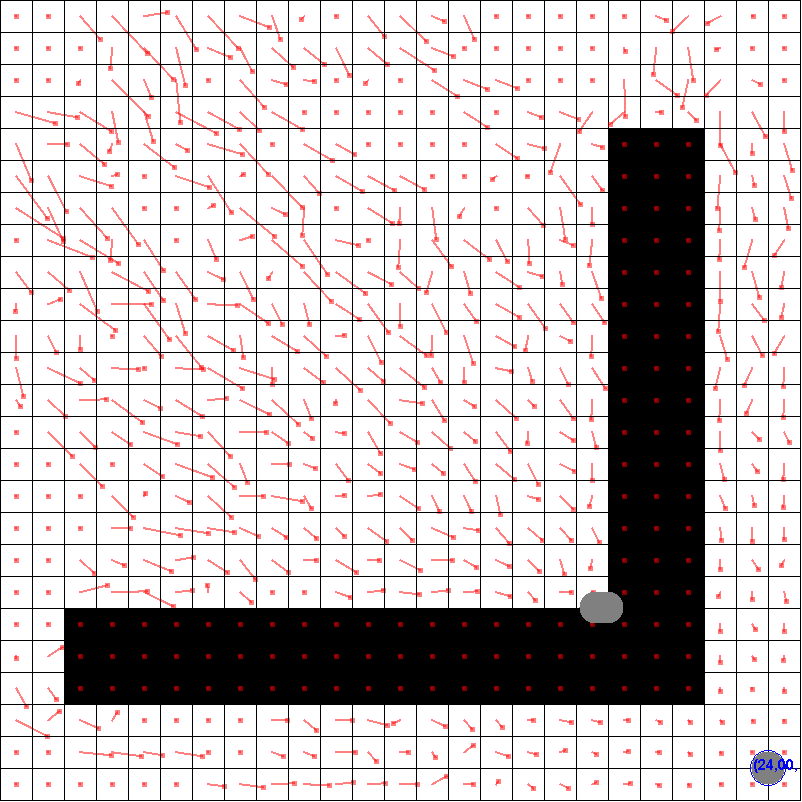
\includegraphics[width=0.3\textwidth]{obstaculos/obstaculo3_inicio_tras_600_iteraciones}
	    }
	    \caption{Ejecución con un obstáculo cóncavo}
	    \label{fig:8}
	\end{figure}
